%############################################################################
\section{Implementation}
\label{sec:ap-implementation}
%############################################################################

\AutoProof is implemented as a library in \EVE. The \AutoProof library consists of around 160 classes with a total of more than 25'000 lines of code.
The \AutoProof library only relies on the Eiffel compiler and handles the translation to and from Boogie. In addition there is the user interface code that deals with the user interaction via GUI and command-line, i.e. starting \AutoProof and displaying the results to the user.


%============================================================================
\subsection{Main interface}
%============================================================================

The main interface to \AutoProof is a single class: \e{E2B_AUTOPROOF}. The prefix \e{E2B} stands for \emph{Eiffel to Boogie}\footnote{Eiffel does not support namespaces, the prefix scheme is used to avoid name clashes.}. Figure~\ref{fig:code_ap} shows the minimal code necessary to launch \AutoProof. After creating an instance of the \AutoProof class, clients use the routines \e{add_class} and \e{add_feature} to add classes and routines that should be verified. After adding a notification agent via \e{add_notification}, a call to \e{verify} will start the process of translating the added classes and features to Boogie and starts the verification. Once the verification is finished, the notification agent will be called with a result object of type \e{E2B_RESULT}. The result object contains a list of verification results of both successful and failed verifications, and possibly a list of semantic and execution errors.

\begin{efigure}[!htb]{Minimal code to run \AutoProof}{fig:code_ap}
	verify_class (a_class: CLASS_C)
			-- Verify class `a_class' with AutoProof.
		local
			autoproof: E2B_AUTOPROOF
		do
			create autoproof.make
			autoproof.add_class (a_class)
			autoproof.add_notification (agent notify)
			autoproof.verify
		end

	notify (a_result: E2B_RESULT)
			-- Handle result from AutoProof.
		do
			-- evaluate result
		end
\end{efigure}


%============================================================================
\subsection{Verification task}
%============================================================================

Internally \AutoProof uses the EiffelStudio ROTA task system, which allows to run tasks asynchronously without the use of multithreading. This is achieved by breaking the implementation of tasks down to small steps that are called during the idle time of the application. The ROTA system is executed in the user interface loop, making it important to keep the processing time of each individual step to a minimum as otherwise the user interface will block during the execution of \AutoProof. Using the ROTA task system instead of real threads is necessary though as the core compiler data structures that \AutoProof used during the translation to Boogie are not thread safe. Using the ROTA system guarantees that no race conditions occur.

\begin{figure}[!htb]
\begin{center}
\includegraphics[width=\columnwidth,page=2]{images/drawings.pdf}
\end{center}
\caption{Workflow of verification main tasks and sub-tasks.}
\label{fig:ap-tasks}
\end{figure}

Figure~\ref{fig:ap-tasks} shows the \AutoProof tasks and their relationship.
There are two different high-level verification tasks in \AutoProof and both are split into the same subtasks. 
The two main tasks---\emph{bulk verification} and \emph{forked verification}---differ in the way they handle the granularity of the Boogie verification. 
In bulk mode all input is translated into a single Boogie file; results are fed back to users when verification of the whole input has completed.
Using \AutoProof in bulk mode minimizes translation and Boogie invocation overhead but provides feedback synchronously, only when the whole batch has been processed.
In contrast, forked mode offers asynchronous feedback: each input routine (and implicit proof obligations such as class invariant admissibility checking) is translated into its own self-contained Boogie file; parallel instances of Boogie run on each file and results are fed back to users asynchronously as soon as any Boogie process terminates.

Both types of main tasks use the same sub-tasks to do the actual verification:
\begin{enumerate}

\item \emph{Translate chunk}: Translates part of the Eiffel input to an intermediate AST representation of Boogie. This task is executed as many times as necessary to translate the whole input.

\item \emph{Generate Boogie}: Takes the intermediate AST and generates Boogie code from it. This Boogie code is combined with the background theory to a single Boogie file.

\item \emph{Execute Boogie}: Executes Boogie on the generated file and waits for its termination. The Boogie process is spawned in a separate process.

\item \emph{Evaluate Boogie}: Evaluates the output from Boogie, traces the findings back to Eiffel, and builds the result object.

\item \emph{Verify with inlining}: If two-step verification is enabled and there where verification errors, this task restarts the verification of the failed routines with inlining and unrolling enabled by going back to the \emph{translate chunk} task.

\item \emph{Merge results}: This task combines the results of two runs of two-step verification.

\item \emph{Notify}: Finally, this task notifies the client of \AutoProof by calling the notification agents with the verification result.

\end{enumerate}


%============================================================================
\subsection{Intermediate AST}
%============================================================================

For the translation of Eiffel to Boogie, \AutoProof uses an intermediate abstract syntax tree (AST).
The intermediate AST models an intermediate verification language like Boogie. The AST contains top-level \emph{declarations} of variables, constants, functions, axioms, procedures and procedure bodies.
Procedure bodies contain \emph{statements} like assertions, assignments, procedure calls, and so on.
Many statements and top-level declarations are composed of \emph{expressions}: values, operations, function calls, quantifiers, and more.
This part of the \AutoProof library is self-contained and could be used by other tools to generate Boogie code.

Using an intermediate AST serves multiple goals:
\begin{enumerate}

\item Making the implementation of the translation from Eiffel simpler.

\item Making it easier to react to changes in the Boogie verifier.

\item Making it possible to implement operations on the intermediate AST.

\end{enumerate}

The first goal has been clearly met. By building an AST, the code of the translator classes are more readable and maintainable, as the programmer is free to think about the generated program in abstract terms, and does not have to take specific syntax or matching braces into account. The alternative---generating Boogie code directly---quickly becomes unmanageable (a previous version of \AutoProof did generate Boogie code directly).

The second goal has been successfully met as well. Since the generation of Boogie code from the intermediate AST is concentrated in a single class it is not difficult to react to changes or extensions in the Boogie syntax.

The last goal is possible with the current design, although it is not being exploited actively at the moment.


%============================================================================
\subsection{Translating Eiffel}
%============================================================================

\begin{figure}[!htb]
\begin{center}
\includegraphics[width=\columnwidth,page=3]{images/drawings.pdf}
\end{center}
\caption{Translation workflow using a translation pool.}
\label{fig:ap-translation-workflow}
\end{figure}

The key task of \AutoProof is translating Eiffel to the intermediate AST representation. For this, \AutoProof uses the notion of \emph{translation unit} and \emph{translation pool}. A translation unit represents an item that needs to be translated from Eiffel to Boogie and the translation pool keeps track of all translation units that need to be translated or are already translated.

The general translation workflow is shown in Figure~\ref{fig:ap-translation-workflow}. The process is started by adding the user input (dark blue shapes) from the Eiffel universe to the translation pool; for all routines that are going to be verified, the intermediate AST representation of the signature and implementation of the routine will be generated (dark red shapes). To do this, the translator (1) takes out one untranslated unit from the pool, (2) generates the intermediate AST representation of that unit, (3) marks the translation unit as translated, and finally (4) if there are untranslated units left in the pool goes back to (1). When the translator encounters an Eiffel routine call, an attribute access, or use of an Eiffel type (e.g. as the type of a local variable), that information of the Eiffel universe needs to be translated as well. These elements are added to the translation pool whenever needed. For routine calls only the signature of the routine will be translated, as \AutoProof does modular verification. Through this process the translation pool grows until the transitive closure of the signature of referenced features is reached.

The different translation units in \AutoProof are:
\begin{itemize}
\item \emph{Type}: generates type constant and inheritance axioms for an Eiffel type.
\item \emph{Class}: generates the invariant admissibility check for an Eiffel class.
\item \emph{Invariant}: generates the invariant predicate and corresponding axioms for an Eiffel type.
\item \emph{Attribute}: generates field constant for an Eiffel attribute and additional axioms depending on the type of the attribute.
\item \emph{Routine signature}: generates the signature of a regular Eiffel routine.
\item \emph{Routine implementation}: generates the implementation of a regular Eiffel routine.
\item \emph{Creator signature}: generates the signature of an Eiffel creation routine.
\item \emph{Creator implementation}: generates the implementation of an Eiffel creation routine.
\item \emph{Functional routine}: generates a Boogie function and corresponding axioms for a pure Eiffel function.
\item \emph{Precondition predicate}: generates a predicate and corresponding axioms for the precondition of an Eiffel routine.
\item \emph{Postcondition predicate}: generates a predicate and corresponding axioms for the postcondition of an Eiffel routine.
\item \emph{Logical signature}: generates the signature of a logical routine.
\item \emph{Contract check}: generates a check for the validity of the read frame or write frame of an Eiffel routine.
\item \emph{Read frame}: generates a Boogie function for the read frame of an Eiffel routine.
\item \emph{Write frame}: generates a Boogie function for the write frame of an Eiffel routine.
\item \emph{Variants}: generates a Boogie function for the decreases function of a recursive Eiffel routine.
\end{itemize}


%============================================================================
\subsection{Interaction with Boogie}
%============================================================================

Once the Eiffel code is translated to the intermediate AST, we can generate the Boogie file and launch the Boogie verifier. We use the visitor pattern~\cite{GAMMA95} to generate the Boogie code; the visitor traverses the AST and generates the appropriate Boogie code for each AST node. The generated Boogie code is prepended with the background theory file that contains the basic definitions and axioms and is written to a file.

Launching the Boogie verifier is done through \e{E2B_EXECUTABLE}, an abstract class that can be implemented through different execution schemes. The standard way of using Boogie is by launching it as a separate process. In addition, we have implemented a remote execution, where the Boogie file is sent over the network to a server which launches Boogie, and then sends back the result. Boogie files are generally quite small and do not take long to send over the network, verification on the other hand can be resource-intensive, this could make it beneficial to run the verification for multiple users on a server instead of the user machine.

When Boogie finishes, \AutoProof parses the output and generates an \e{E2B_RESULT} object and returns it to the client of \AutoProof.


%============================================================================
\subsection{Tracing result to Eiffel}
%============================================================================

In order to trace Boogie errors to the originating Eiffel source code, \AutoProof uses structured names for Boogie procedures and inserts structured comments into the Boogie code. For an Eiffel routine \e{r} in class \e{C}, the Boogie procedure generated for verifying this Eiffel routine is called \b{C.r}\footnote{Boogie allows symbols such as the dot or hash in identifiers} and for each assertion that is generated in the Boogie code a structured comment similar to the following comment is appended:

\begin{brunning}
 // type:termination tag:variant_decreases line:138
\end{brunning}

When Boogie reports its results, the Boogie procedure name can be parsed and mapped to the original Eiffel routine. For each assertion violation the Boogie source code is used to read the type of assertion and other available information such as line number. In addition to \emph{type}, \emph{tag}, and \emph{line}, the assertion comments can also contain information about called routines (for precondition violations) or if an assertion was automatically generated (e.g for semantic collaboration defaults). \AutoProof displays this information through the user interface and in the error message.

\AutoProof has a feature of associating a result handler (in form of an Eiffel agent) for any Boogie procedure in addition to using structured Boogie procedure names. When the Boogie result is available and a result handler is associated with the corresponding Boogie procedure, \AutoProof will notify the result handler. This mechanism is used for certain verifications that are not directly related to an Eiffel routine like the admissibility check for class invariants.


%============================================================================
\subsection{Extending \AutoProof}
%============================================================================

\AutoProof has been built with extendibility in mind. It offers multiple features to extend the translation to Boogie, with or without having to touch the actual implementation.

%----------------------------------------------------------------------------
\subsubsection{Boogie mapping}
%----------------------------------------------------------------------------

Classes can specify a Boogie file that should be included in the generated Boogie file whenever an entity of this class is used. This allows to include an axiomatization or background theory related to a specific class. In addition, a per class option allows to map an Eiffel type to a Boogie type and a per routine option allows to map Eiffel functions to Boogie functions. This Boogie mapping is used to axiomatize and translate the MML library.

%----------------------------------------------------------------------------
\subsubsection{Extension points}
%----------------------------------------------------------------------------

\AutoProof offers three extension points: \emph{calls}, \emph{nested expressions}, and \emph{across expressions}. Handlers can be registered for each extension point. When the translator hits one of the extension points in the traversal of the Eiffel AST it will call each registered handler in a chain of responsibility style~\cite{GAMMA95}. The first handler that replies positively will do the translation and if no handler accepts the default translation will continue. The three extension points are:

\begin{itemize}

\item The \emph{call} extension point triggers at every routine call. The information provided to the handler are the target and called routine. When the handler does the translation of the call to Boogie it is also its responsibility to translate the arguments of the call, though the handler can delegate the translation of subexpressions like the arguments back to the default translator.

\item The \emph{nested expression} extension point triggers at every nested expression. Given the AST node, the handler can inspect the AST surrounding the nested expression to decide if it wants to handle the expression. This extension point is more general than the \emph{call} extension point but harder to use.

\item The \emph{across expression} extension point triggers at across expressions (but not at across loop statements). This is an important extension point for \AutoProof, as it allows to implement translations for universal and existential quantifiers. The handler will be called for multiple points in the translation, first to set up the quantifier and then for each time the internal cursor is used (e.g. for calls to \e{item}).

\end{itemize}

Extension points are used in \AutoProof for special translations of built-in features and several base library features. Table~\ref{tab:extensions} gives an overview of implemented extension handlers, and what they are used for.

\begin{table}[htb]
\begin{tabular}{llp{7.5cm}}
Target & Type & Purpose \\
\hline 
\e{ANY} & call / nested & Special translation for a few routines of class \e{ANY}. \\
\e{TYPE} & call / nested & Special translation for a few routines of class \e{TYPE}. \\
\e{NUMERIC} & call & Map several functions of numeric types (integers and reals) to Boogie functions from the background theory. \\
Logical & call / nested & Use functions from the background theory for operations involving MML classes (e.g. equality comparison). \\
Ownership & call & Implements special handling for ghost features involved in ownership and semantic collaboration. \\
\e{MML} & across & Use MML types in across expressions. \\
\e{INTERVAL} & across & Use integer intervals in across expressions. \\
\e{SIMPLE_ARRAY} & across & Use \e{SIMPLE_ARRAY} in across expressions. \\
\e{SIMPLE_LIST} & across & Use \e{SIMPLE_LIST} in across expressions. \\
\end{tabular}
\caption{Implemented handlers for extension points.}
\label{tab:extensions}
\end{table}




